\documentclass[12pt,reqno]{article}
\usepackage[dutch]{babel}
\usepackage[margin=1.2in]{geometry}
\usepackage{amsmath}
\usepackage{amssymb}
\usepackage{amsthm}
\usepackage{color}
\usepackage{tikz}
\usepackage{url}

\title{\textbf{Congruente getallen}}
\author{
	\begin{tabular}{ l l }
		Lotte Bruijnen, & 4297652 \\
		Daan van Laar, & 5518741 \\
		Suzanne Vincken, & 4273338
	\end{tabular}\\\\
	Onder begeleiding van: Carel Faber, UU
}
\date{04-01-2016}

\newcommand*{\NN}{\ensuremath{\mathbb{N}}}
\newcommand*{\ZZ}{\ensuremath{\mathbb{Z}}}
\newcommand*{\QQ}{\ensuremath{\mathbb{Q}}}
\newcommand*{\RR}{\ensuremath{\mathbb{R}}}
\newcommand*{\CC}{\ensuremath{\mathbb{C}}}
\newcommand*{\NO}{\ensuremath{\mathbb{N}_{>0}}}

\renewcommand{\qedsymbol}{$\blacksquare$}

\theoremstyle{theorem}
\newtheorem{theorem}{Stelling}
\newtheorem{lemma}[theorem]{Lemma}
\newtheorem{proposition}[theorem]{Propositie}
\newtheorem{corollary}[theorem]{Gevolg}

\theoremstyle{definition}
\newtheorem{example}[theorem]{Voorbeeld}
\newtheorem{definition}[theorem]{Definitie}
\newtheorem{remark}[theorem]{Opmerking}

\DeclareMathOperator{\ggd}{ggd}

\hyphenation{Pytha-go-reïsch}
\hyphenation{pytha-go-reïsch}
\hyphenation{Mathematics}

\begin{document}
	\begin{titlepage}
		\maketitle
		\thispagestyle{empty}
		\begin{figure*}[h!]
			\centering
			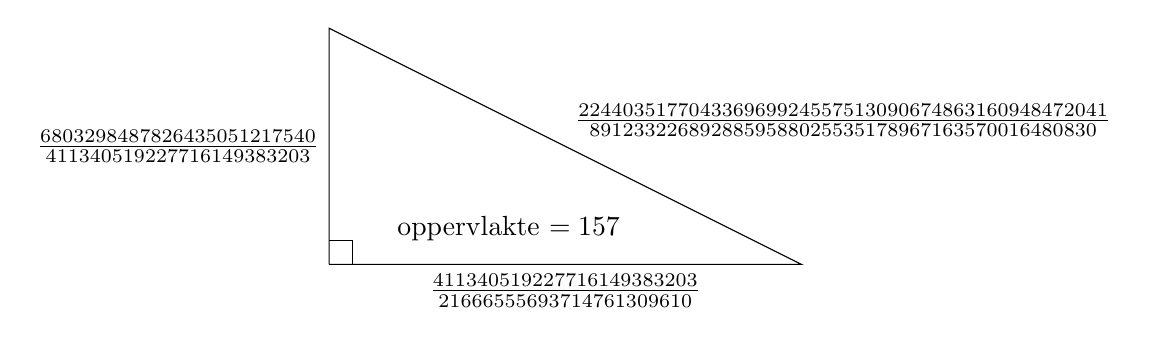
\begin{tikzpicture}[xscale=6, yscale=3]
			\coordinate (O) at (0,0);
			\coordinate (A) at (1,0);
			\coordinate (B) at (0,1);
			\coordinate (M) at (0.38, 0.15);
			\draw (O) -- node[auto,swap]{$\frac{411340519227716149383203}{21666555693714761309610}$} 
			(A) -- node[auto,swap]{$\frac{224403517704336969924557513090674863160948472041}{8912332268928859588025535178967163570016480830}$}
			(B) -- node[auto,swap]{$\frac{6803298487826435051217540}{411340519227716149383203}$} (O);
			\draw (M) node[auto]{oppervlakte $=157$};
			\coordinate (X1) at (0,0.1);
			\coordinate (X2) at (0.05,0.1);
			\coordinate (X3) at (0.05,0);
			\draw (X1) -- (X2) -- (X3);
			\end{tikzpicture}
		\end{figure*}
	\end{titlepage}

	\allowdisplaybreaks
	
	\section{Inleiding}
	We hebben onderzoek gedaan naar congruente getallen om onze kennis te verbreden. Het is een onderwerp uit de getaltheorie. In dit werkstuk zullen we vertellen wat we hebben gevonden.
	
	In hoofdstuk \ref{sec:def} zullen we Pythagore\"ische drietallen en congruente getallen behandelen. We zullen definities geven en we leggen uit wat deze twee onderwerpen met elkaar te maken hebben. Daarna, in hoofdstuk \ref{sec:vb}, zullen we een aantal voorbeelden geven van congruente getallen. Hoofdstuk \ref{sec:suus} zal gaan over het vinden van congruente getallen. Hoe vinden we alle getallen die congruent zijn? In het laatste hoofdstuk, hoofdstuk \ref{sec:lotte}, zullen we kijken naar presentaties van congruente getallen. Dit heeft te maken met Pythagore\"ische drietallen. Als afsluiting zullen we een samenvatting geven van alles wat we hebben behandeld.
	
	
	%\beginsection{Daan}
	\section{Pythagore\"ische drietallen en congruente getallen}\label{sec:def}
	%Wat is een Pythagoreisch drietal?
	%Wat is een congruent getal?
	%  - algebraische definitie + bewijs
	%  - meetkundige definitie
	%  - equivalentie van die twee definities
	%  - definitie primitieve congruente getallen: Een kwadraatvrij congruent getal
	%Er schijnt een stelling te zijn die alle Pythagoreïsche drietallen classificeert. Als je die kan vinden, kan je het die even noemen.
	Eerst zullen we kijken naar de definitie van congruente getallen. Er bestaan echter meerdere definities. We zullen er hier twee behandelen.\\
	
	Ten eerste kijken we naar de meetkundige definitie uit \cite{Oort}[p.3]:	
	\begin{definition}\label{def:meetkunde}
		Een positief geheel getal $n$ heet een congruent getal als er een rechthoekige driehoek bestaat met lengtes van zijden in $\QQ_{>0}$ en met oppervlak gelijk aan $n$. Noem de lengtes van de zijden $x,y,z\in\QQ$; met behulp van de stelling van Pythagoras \textcolor{red}{en de formule voor de oppervlakte van een driehoek} zien we:
		\begin{figure*}[h!]
			\centering
			\begin{tikzpicture}[xscale=6, yscale=3]
			\coordinate (O) at (0,0);
			\coordinate (A) at (1,0);
			\coordinate (B) at (0,1);
			\draw (O) -- node[auto,swap]{$x$} 
			(A) -- node[auto,swap]{$z$}
			(B) -- node[auto,swap]{$y$} (O);
			\coordinate (M) at (1.5, 0.5);
			\draw (M) node[auto]{$x\cdot \dfrac{y}{2} = n$};
			\coordinate (N) at (1.5, 0.25);
			\draw (N) node[auto]{$x^2 + y^2 = z^2$};
			\coordinate (X1) at (0,0.1);
			\coordinate (X2) at (0.05,0.1);
			\coordinate (X3) at (0.05,0);
			\draw (X1) -- (X2) -- (X3);
			\end{tikzpicture}
		\end{figure*}
	\end{definition}
	We zien dat hier een congruent getal $n$ wordt gegeven als de oppervlakte van een rechthoekige driehoek waarvan (de lengte van) de zijden in $\QQ$ zitten. \textcolor{red}{Grammaticaal beetje iffy, kan wel overigens} We kunnen conguente getallen ook bekijken via een algebra\"{i}sche benadering. De volgende definitie komt van \cite{Oort}[p.3].
	
	\begin{definition}\label{def:algebra}
		Een positief geheel getal $n$ heet een congruent getal als er een $\delta\in\QQ$ bestaat zodanig dat
		\begin{equation*}
			\delta^2 - n,\quad \delta^2,\quad \delta^2 + n
		\end{equation*}
		kwadraten zijn in $\QQ$. \textcolor{red}{Maak duidelijk dat het kwadraten van rationale getallen zijn!}
	\end{definition}	
	Een getal dat aan deze definitie voldoet is het getal 5. We nemen $\delta = \frac{41}{12}$. Dan geldt:
	\begin{align*}
		\delta^2 &= \left( \frac{41}{12} \right)^2 \in\QQ \\
		\delta^2 - n &= \frac{1681}{144} - 5 = \frac{961}{144} = \left( \frac{31}{12} \right)^2 \in\QQ \\
		\delta^2 + n &= \frac{1681}{144} + 5 = \frac{2401}{144} = \left( \frac{49}{12} \right)^2 \in\QQ
	\end{align*}
	Hieruit volgt dus dat $5$ een conguent getal is. \\
	
	Dit lijken twee onafhankelijke definities te zijn, maar ze zijn in feite equivalent. Dit gaan we op de volgende manier bewijzen: \\
	
	\begin{proposition}
		\cite{Koblitz}[p.4, vertaald] Laat $n$ een vast kwadraatvrij positief getal zijn. Laat $x,y,z,\delta \in\QQ$ met $x<y<z$. Er is een \'e\'en op \'e\'en relatie tussen rechthoekige driehoeken met zijden $x$ en $y$, schuine zijde $z$ en oppervlakte $n$, en getallen $\delta$ waarvoor geldt dat $\delta$, $\delta +n$ en $\delta -n$ de kwadraten zijn van een rationaal getal. De correspondentie is:
		\begin{align}
			x,y,z &\rightarrow \delta = \left( \frac{z}{2} \right)^2 \\
			\delta &\rightarrow x=\sqrt{\delta+n} - \sqrt{\delta-n},\quad y = \sqrt{\delta+n}+\sqrt{\delta-n},\quad z = 2\sqrt{\delta}.
		\end{align}
		In het bijzonder, $n$ is een congruent getal dan en slechts dan als er een $\delta$ bestaat z\'o dat $\delta$, $\delta+n$ en $\delta-n$ kwadraten van rationale getallen zijn.
	\end{proposition}
	\begin{proof}
		We beginnen door een drietal $(x,y,z)$ te nemen met de gewenste eigenschappen, dus
		\begin{equation*}
			x^2 + y^2 = z^2 \text{ en } \frac{1}{2}xy=n
		\end{equation*}
		Als we 4 keer de tweede vergelijking van de eerste afhalen of erbij optellen houden we het volgende over:
		\begin{align*}
			x^2 \pm 2xy + y^2 = z^2 \pm 4n \\
			(x \pm y)^2 = z^2 \pm 4n
		\end{align*}
		Door nu beide kanten door 4 te delen kunnen we eenvoudig zien dat $\delta = (\frac{z}{2})^2$ de eigenschap heeft dat $\delta \pm n$ rationale kwadraten zijn
	\end{proof}
	Hieruit volgt dat de twee eerder gegeven definities in feite equivalent zijn aan elkaar. Het maakt niet heel veel uit welke definitie wij zullen hanteren, maar voor het gemak gaan we uit van definitie 1. \\
	
	Bij de eerste definitie maken we gebruik van Pythagore\"ische drietallen. Daar zullen we nu wat meer over uitleggen.\\
	
	De geschiedenis van Pythagore\"ische drietallen begint bij het vermoeden van Fermat. De bijbehorende vergelijking is als volgt geformuleerd:
	\begin{equation}\label{fermat}
		x^n + y^n = z^n \qquad \text{met} \qquad n \in \NN.
	\end{equation}
	Fermat vermoedde dat voor $n \geq 3$ er alleen triviale oplossingen bestaan voor (\ref{fermat}) \textcolor{red}{Zin loopt een beetje moeizaam. Kijk of je 'm kan herschrijven}. Dat wil zeggen, $\forall (x,y,z) \in \ZZ^3$ en $x^n + y^n = z^n$ met $n \geq 3$ en $x, y, z \geq 0$, geldt $x \cdot y \cdot z = 0$. \\
	Wij zijn echter vooral ge\"interesseerd in het geval waarbij $n=2$ en alle niet triviale oplossingen van de vergelijking $x^2 + y^2 = z^2$. Deze oplossingen noteren we als $(x,y,z)$ en we noemen deze oplossingen Pythagore\"ische drietallen. Dit komt omdat het vermoeden van Fermat met $n=2$ de stelling van Pythagoras is. \textcolor{red}{In zijn commentaar wordt dit door Faber in twijfel getrokken} De niet-triviale oplossingen $(x,y,z)$ van $x^2 + y^2 = z^2$ vormen dan ook een rechthoekige driehoek waarbij $z$ de schuine zijde is. Een simpel voorbeeld van een Pythagore\"isch drietal is $(3,4,5)$, want $3^2 + 4^2 = 9 + 16 = 25 = 5^2$. \\
	Een speciaal soort Pythagore\"isch drietal is het zogenaamde primitieve \mbox{Pythagore\"ische} drietal. Dit is een Pythagore\"isch drietal $(x,y,z)$ waarvoor ook geldt dat de grootste gemeenschappelijke deler van x en y 1 is. \textcolor{red}{Zet x en y tussen dollartekens, zodat ze cursief staan} We noteren dit als $\ggd(x,y) = 1$. Nu kunnen en gaan we het volgende bewijzen: \textcolor{red}{Kies een persoonsvorm, bij voorkeur "kunnen".}
	
	\begin{theorem}
		Als $(x,y,z)$ een Pythagore\"isch drietal is met $\ggd(x,y) = 1$, dan $\ggd(x,z) = 1$.
	\end{theorem}
	\begin{proof}
		Stel, $\ggd(x,z) = d \geq 1$. Dan deelt $d$ zowel $x$ als $y$. Hieruit kunnen we als volgt concluderen dat $y$ ook door $d$ wordt gedeeld:
		\begin{align*}
			d\mid x \text{ en } d\mid z \\
			d^2\mid x^2 \text{ en } d^2 \mid z^2 \\
			d^2\mid z^2 - x^2 \text{ (want } z>x \text{)} \\
			\text{dus, } d^2 \mid y^2 \text{ (uit $x^2 + y^2 = z^2$ volgt $y^2 = z^2 - x^2$)} \\
			\text{dus, } d \mid y \\
			\text{dus, } \ggd(x, y) \geq d \geq 1
		\end{align*}
		Stel nu dat $\ggd(x, y) = 1$. Dit kan alleen zo zijn als $\ggd(x, z) $ ook gelijk aan $1$ is. 
	\end{proof}	
	\textcolor{red}{De opmaak van dit bewijs (vooral de align) is nogal wazig.}
	Verder hebben primitieve Pythagore\"ische drietallen nog veel meer eigenschappen, die elk bewezen kunnen worden. Wij zullen nog een aantal van deze eigenschappen behandelen, te beginnen met welke getallen even, en welke getallen oneven zijn. Van $x$ en $y$ is er altijd \'e\'en getal even. Daardoor is $z$ altijd oneven. \textcolor{red}{Geef duidelijker aan wat precies de stelling is welke je wil bewijzen}
	\begin{proof}
		Voor $x$ en $y$ zijn er 3 \textcolor{red}{drie} mogelijkheden: allebei even, allebei oneven of 1 \textcolor{red}{\'e\'en} van de 2 \textcolor{red}{twee} is even. De eerste mogelijkheid kunnen we snel afschrijven. Als $x$ en $y$ allebei even zouden zijn, dan is $\ggd(x,y) \neq 1$ want 2 is sowieso een deler. Om te bewijzen dat $x$ en $y$ niet allebei oneven kunnen zijn, nemen we eerst aan dat dat wel zo is:
		\begin{align*}
			x = 2s + 1\\
			y = 2t + 1\\
		\end{align*}
		Uitwerken hiervan geeft dat $z^2$ een even getal is, en daarom $z$ ook (het kwadraat van een oneven getal is weer een oneven getal en de som van 2 oneven getallen is weer even). We schrijven $z = 2u$
		\begin{align*}
			x^2 + y^2 = z^2\\
			(2s + 1)^2 + (2t + 1)^2 = (2u)^2\\
			4s^2 + 4s + 1 +4t^2 + 4t + 1 = 4u^2\\
			4(s^2 + s + t^2 + t) + 2 = 4u^2
		\end{align*}
		Als we beide kanten door 4 zouden delen, krijgen we een rest van 2 aan de linkerkant en een rest van 0 aan de rechterkant. Dit kan natuurlijk niet, dus $x$ en $y$ zijn niet allebei oneven. \\
		We kunnen nu concluderen dat $x$ en $y$ niet allebei even zijn, en ook niet allebei oneven zijn. Een van de getallen $x$ of $y$ moet dus per definitie oneven zijn en de ander moet per definitie even zijn. Hieruit volgt dat $z$ altijd een oneven getal is. $x^2$ is namelijk even en $y^2$ is oneven (of precies andersom, zonder verlies van algemeenheid). De som van een oneven en een even getal is een oneven getal, waardoor $z^2$ en $z$ oneven zijn.
	\end{proof}
	Een derde eigenschap van een Pythagore\"isch drietal is dat $\frac{(z-x)(z-y)}{2}$ een kwadraat is. \cite{Posamentier}[p.156]
	
	%\endsection{Daan}


	\section{Voorbeelden}\label{sec:vb}
	De eerste negentien congruente getallen zijn: $5$, $6$, $7$, $13$, $14$, $15$, $21$, $22$, $23$, $29$, $30$, $31$, $34$, $37$, $38$, $39$, $41$, $46$, $47$, zie \cite{Coates}[p.19]. We zullen hieronder drie voorbeelden geven. Daarna zullen we bewijzen dat $n=1$ geen congruent getal is.\\
	\\
	Het kleinste congruente getal is $5$. Dat correspondeert met de driehoek met de volgende zijden:
	\begin{figure*}[h!]
		\centering
		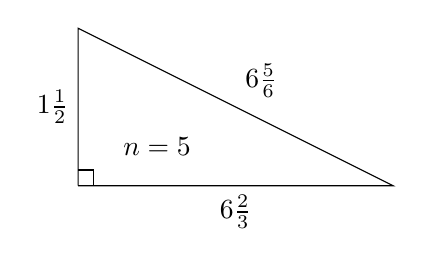
\begin{tikzpicture}[xscale=4, yscale=2]
		\coordinate (O) at (0,0);
		\coordinate (A) at (1,0);
		\coordinate (B) at (0,1);
		\coordinate (M) at (0.25, 0.25);
		\draw (O) -- node[auto,swap]{$6\frac{2}{3}$} 
		(A) -- node[auto,swap]{$6\frac{5}{6}$}
		(B) -- node[auto,swap]{$1\frac{1}{2}$} (O);
		\draw (M) node[auto]{$n=5$};
		\coordinate (X1) at (0,0.1);
		\coordinate (X2) at (0.05,0.1);
		\coordinate (X3) at (0.05,0);
		\draw (X1) -- (X2) -- (X3);
		\end{tikzpicture}
	\end{figure*}\\
	Het kleinste congruente getal met zijden uit $\NN$ is $6$. Dat correspondeert met de driehoek met de volgende zijden:
	\begin{figure*}[h!]
		\centering
		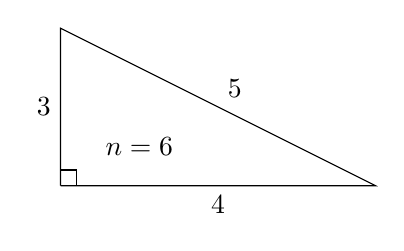
\begin{tikzpicture}[xscale=4, yscale=2]
		\coordinate (O) at (0,0);
		\coordinate (A) at (1,0);
		\coordinate (B) at (0,1);
		\coordinate (M) at (0.25, 0.25);
		\draw (O) -- node[auto,swap]{$4$} 
		(A) -- node[auto,swap]{$5$}
		(B) -- node[auto,swap]{$3$} (O);
		\draw (M) node[auto]{$n=6$};
		\coordinate (X1) at (0,0.1);
		\coordinate (X2) at (0.05,0.1);
		\coordinate (X3) at (0.05,0);
		\draw (X1) -- (X2) -- (X3);
		\end{tikzpicture}
	\end{figure*}\\
	De onderstaande driehoek correspondeert met het congruente getal $n=157$: \cite{Koblitz}[p.5]
	\begin{figure*}[h!]
		\centering
		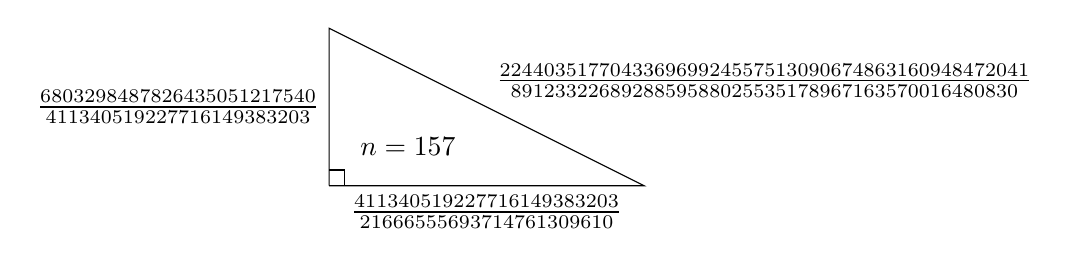
\begin{tikzpicture}[xscale=4, yscale=2]
		\coordinate (O) at (0,0);
		\coordinate (A) at (1,0);
		\coordinate (B) at (0,1);
		\coordinate (M) at (0.25, 0.25);
		\draw (O) -- node[auto,swap]{$\frac{411340519227716149383203}{21666555693714761309610}$} 
		(A) -- node[auto,swap]{$\frac{224403517704336969924557513090674863160948472041}{8912332268928859588025535178967163570016480830}$}
		(B) -- node[auto,swap]{$\frac{6803298487826435051217540}{411340519227716149383203}$} (O);
		\draw (M) node[auto]{$n=157$};
		\coordinate (X1) at (0,0.1);
		\coordinate (X2) at (0.05,0.1);
		\coordinate (X3) at (0.05,0);
		\draw (X1) -- (X2) -- (X3);
		\end{tikzpicture}
	\end{figure*}\\
	
	We zullen hieronder bewijzen dat $n=1$ geen congruent getal is. Daarvoor bekijken we eerst een aantal benodigde stellingen en opmerkingen. Ook hebben we het begrip ``relatief priem" nodig: als twee getallen relatief priem zijn, wil dat zeggen dat ze geen factoren gemeen hebben, oftewel hun grootste gemene deler is 1.
	
	\begin{theorem}\label{1:hulp2}
		Twee positieve gehele getallen die relatief priem zijn en waarvan het product een kwadraat is, moeten zelf kwadraten zijn.
	\end{theorem}
	\begin{proof}
		Neem $x,y\in\NO$ met $\ggd(x,y) = 1$. Stel dat $xy$ een kwadraat is. Laat nu $p$ een priemfactor zijn van $x$, maar niet van $y$. Dan weten we dat $p$ in tweevoud moet voorkomen in $xy$, omdat $xy$ een kwadraat is en omdat $p$ niet in $y$ voorkomt. Hierdoor weten we ook dat $p$ in tweevoud moet voorkomen in $x$. Dus $x$ is een kwadraat. We kunnen dit op dezelfde manier doen voor $y$, dus $y$ is een kwadraat. Merk op dat in het bijzonder $x$ of $y$ ook $1$ zouden kunnen zijn. Hiermee is de stelling bewezen.
	\end{proof}
	
	\begin{remark}\label{1:hulp4}
		Merk op dat als $xy$ een vierde macht is, dan zijn $x$ en $y$ ook vierde machten. We kunnen dit op dezelfde manier doen als bij stelling \ref{1:hulp2}. Laat $p$ een priemfactor zijn van $x$, maar niet van $y$. Dan weten we dat $p$ in viervoud moet voorkomen in $xy$, omdat $xy$ een vierde macht is en omdat $p$ niet in $y$ voorkomt. Hierdoor weten we ook dat $p$ in viervoud moet voorkomen in $x$. Dus $x$ is een vierde macht. We kunnen dit op dezelfde manier doen voor $y$, dus $y$ is een vierde macht.
	\end{remark}
	
	We moeten nu ook nog iets weten over modulo rekenen.
	\begin{remark}\label{1:hulpMod}
		Een even kwadraat is altijd $0 \pmod{4}$. Namelijk; een even getal is $0,2 \pmod{4}$, dus een even kwadraat is $0^2 \equiv 2^2 \equiv 0 \pmod{4}$. Een oneven kwadraat is altijd $1 \pmod{4}$. Namelijk; een oneven getal is $1,3 \pmod{4}$, dus een oneven kwadraat is $1^2 \equiv 3^2 \equiv 1 \pmod{4}$.
	\end{remark}
		
	We zullen nu de onderstaande stelling bewijzen.
	\begin{theorem}
		Het getal $n=1$ is geen congruent getal.
	\end{theorem}
	\begin{proof}
		Voor dit bewijs hebben we gebruik gemaakt van \cite{Conrad}[p.3-4].\\
		Stel we hebben een rechthoekige driehoek met oppervlakte $1$. We noemen de zijden $\frac{a}{d}, \frac{b}{d}, \frac{c}{d}$ met $a,b,c,d\in\NO$. We kunnen nu alle zijden met $d$ vermenigvuldigen, dan geldt er $a^2 + b^2 = c ^2$ en $\frac{1}{2}ab = d^2$. Als we de tweede vergelijking omschrijven, geeft dat ons de volgende vergelijkingen:
		\begin{equation}\label{1:gedefineerd}
			a^2 + b^2 = c^2 \quad \text{en} \quad ab = 2d^2.
		\end{equation}
		We gaan laten zien dat (\ref{1:gedefineerd}) geen gehele positieve oplossingen heeft.\\
		
		Stel dat (\ref{1:gedefineerd}) een oplossing heeft in $\NO$, zeg $(a, b, c, d)$. Dan zullen we nu bewijzen dat er een oplossing is zodat $a$ en $b$ relatief priem zijn. Stel $\ggd(a,b) = g$. Dan weten we dat $g \mid a$ en $g \mid b$. Hieruit volgen twee resultaten samen met (\ref{1:gedefineerd}). Ten eerste weten we dat $g^2 \mid a^2$ en $g^2 \mid b^2$. Hieruit volgt dat $g^2 \mid a^2 + b^2$, dus $g^2 \mid c^2$, wat betekent dat $g \mid c$. Ten tweede weten we dat $g^2 \mid ab$, dus $g^2 \mid 2d^2$, waaruit volgt dat $g^2 \mid d^2$, met de volgende reden: Omdat $g^2 \mid 2d^2$, weten we dat $2\frac{d^2}{g^2} = x \in\NN$. Omdat $\frac{d^2}{g^2}$ een kwadraat is, weten we dat het een even aantal factoren $2$ bevat (omdat $\frac{d^2}{g^2}\in\QQ$ kan dit in principe ook een negatief aantal factoren 2 zijn). Dan bevat $2\frac{d^2}{g^2} = x$ dus een oneven aantal factoren $2$. Omdat er geldt dat $x \in\NN$ en omdat het een oneven aantal factoren 2 heeft, is $x$ een even getal. We kunnen de vergelijking aan beide kanten door $2$ delen. Dit geeft ons $\frac{d^2}{g^2}=\frac{x}{2} \in\NN$. Dus $g^2 \mid d^2$. Hieruit volgt dat $g \mid d$. We weten nu dus dat $g \mid a$, $g \mid b$, $g \mid c$ en $g \mid d$. We kunnen dus alle zijden door $g$ delen zodat we $a'$, $b'$, $c'$ en $d'$ krijgen die voldoen aan (\ref{1:gedefineerd}) met $\ggd(a',b') = 1$. Er is dus een oplossing $(a,b,c,d)$ voor vergelijking (\ref{1:gedefineerd}), zodat $\ggd(a,b)=1$. We gaan nu verder met bewijzen dat (\ref{1:gedefineerd}) geen gehele positieve oplossingen heeft, met de extra voorwaarde dat $\ggd(a,b) = 1$.\\
		
		Laat $(a, b, c, d)$ een oplossing zijn met $\ggd(a,b) = 1$ en $c$ minimaal. Om te bewijzen dat de stelling waar is, zullen een nieuw viertal $a', b', c', d' \in\NO$ construeren, die voldoet aan (\ref{1:gedefineerd}) met $\ggd(a',b') = 1$ en $0 < c' < c$. Dit geeft een tegenspraak met de aanname dat $c$ minimaal is.\\
		
		Er geldt dat $ab = 2d^2$ en $\ggd(a,b)=1$, waardoor we weten dat $a$ \'of $b$ even is, maar niet beide. Hieruit volgt dat $c^2 = a^2 + b^2$ oneven is, waaruit volgt dat $c$ oneven is. We kunnen zonder verlies van algemeenheid zeggen dat $a$ even en dat $b$ oneven is. We kunnen, vanwege stelling \ref{1:hulp2}, nu stellen dat
		\begin{equation*}
			a = 2k^2 \quad \text{en} \quad b = l^2
		\end{equation*}
		voor $k,l\in\NO$ met $l$ oneven (omdat $b$ oneven is). Als we $a = 2k^2$ invullen in (\ref{1:gedefineerd}), krijgen we de vergelijking $4k^4 + b^2 = c^2$. Hieruit volgt, door factorisatie, dat $k^4 = \frac{c+b}{2}\frac{c-b}{2}$. We weten dat $b$ en $c$ beide oneven en relatief priem zijn, want als $c$ en $b$ niet relatief priem zijn, dan geldt er dat $\ggd(a,b)\neq1$ door $a^2 = c^2 - b^2$. We kunnen nu ook zeggen dat $\frac{c+b}{2}$ en $\frac{c-b}{2}$ relatief priem zijn, want stel $\ggd(\frac{c+b}{2},\frac{c-b}{2})=g$, dan geldt er dat $g$ de som deelt: $g \mid c$ en dat $g$ het verschil deelt: $g \mid b$. Aangezien $\ggd(b,c) = 1$, geldt er ook dat $\ggd(\frac{c+b}{2}, \frac{c-b}{2}) = 1$. We defini\"eren nu
		\begin{equation}\label{1:bc}
			r^4 = \frac{c+b}{2} \quad \text{en} \quad s^4 = \frac{c-b}{2}
		\end{equation}
		voor positieve gehele getallen $r$ en $s$ die relatief priem zijn, dit kan volgens opmerking \ref{1:hulp4}. Er geldt ook dat $r^4$ en $s^4$ relatief priem zijn, dus $r^2$ en $s^2$ zijn relatief priem en ook $r$ en $s$ zijn relatief priem. We lossen nu vergelijking (\ref{1:bc}) op voor $b$ en $c$, wat ons de volgende resultaten geeft:
		\begin{equation*}
			b = r^4 - s^4 \quad \text{en} \quad c = r^4 + s^4,
		\end{equation*}
		waaruit volgt dat $l^2 = b = (r^2 + s^2) (r^2 - s^2)$. De twee factoren $(r^2 + s^2)$ en $(r^2 - s^2)$ zijn relatief priem, want stel dat $ggd(r^2 + s^2, r^2 - s^2) = g$, dan weten we in ieder geval dat $g$ oneven is, omdat $b = r^4 - s^4$ en $c = r^4 + s^4$ oneven zijn. We weten ook dat $g$ de som deelt: $g \mid 2r^2$ en dat $g$ het verschil deelt: $g \mid 2s^2$. Omdat $g$ oneven is, kan $g$ niet $2$ delen, dat betekent dus dat $g \mid r^2$ en $g \mid s^2$, dit is in tegenspraak met het feit dat $\ggd(r^2, s^2) = 1$. Dus de twee factoren $(r^2 + s^2)$ en $(r^2 - s^2)$ zijn relatief priem. De eerste factor, $r^2 + s^2$, is sowieso positief. Omdat het product ook positief is, geldt er dat $r^2 - s^2$ ook positief is. Vanwege stelling \ref{1:hulp2} kunnen we nu schrijven 
		\begin{equation}\label{1:r}
			t^2 = r^2 + s^2 \quad \text{en} \quad u^2 = r^2 - s^2
		\end{equation}
		voor oneven positieve gehele getallen $t$ en $u$, waarvoor geldt dat deze ook relatief priem zijn. We gebruiken nu opmerking \ref{1:hulpMod}; omdat $u$ oneven is, geldt er dat $u^2 \equiv 1 \pmod{4}$, dus $r^2 - s^2 \equiv 1 \pmod{4}$. Hieruit volgt dat $r$ oneven is, dus is $s$ even. Namelijk: Er moet gelden dat $r$ en $s$ verschillende pariteit hebben, want anders geldt er dat $r^2 - s^2 \equiv 0 \pmod{4}$. Stel nu dat $r$ is even, dan is $s$ oneven. Er geldt nu dat $r^2 \equiv 0 \pmod{4}$ en $s^2 \equiv 1 \pmod{4}$. Dit levert op: $r^2 - s^2 \equiv -1 \equiv 3 \pmod{4}$ en dat kan niet. We weten dus dat $r$ oneven is en dat $s$ even is. Nu lossen we  (\ref{1:r}) op voor $r^2$. Dit geeft ons:
		\begin{equation*}
			r^2 = \frac{t^2 + u^2}{2} = \left( \frac{t+u}{2} \right)^2 + \left( \frac{t-u}{2} \right)^2,
		\end{equation*}
		met $\frac{t \pm u}{2} \in\ZZ$ omdat $t$ en $u$ beide oneven zijn. We zien hierboven dus een nieuwe, kleinere, oplossing voor vergelijking (\ref{1:gedefineerd}). We defini\"eren
		\begin{equation*}
			a' = \frac{t+u}{2}, \quad b' = \frac{t-u}{2} \quad \text{en} \quad c' = r.
		\end{equation*}
		Er geldt dat $\ggd(a',b') = 1$, om dezelfde reden dat de eerder genoemde factoren $\frac{c+b}{2}$ en $\frac{c-b}{2}$ relatief priem zijn. Als we gebruik maken van (\ref{1:r}), vinden we dat $a'b' = \frac{t^2 - u^2}{4} = \frac{2s^2}{4} = 2\left( \frac{s}{2} \right)^2$. Laat $d' = \frac{s}{2} \in\ZZ$, dan hebben we nu een nieuwe oplossing $(a', b', c', d')$ voor (\ref{1:gedefineerd}). Er geldt dat $0 < c'= r \leq r^4 < r^4 + s^4 = c$. Dit geeft een tegenspraak, omdat $c$ minimaal is. Dus (\ref{1:gedefineerd}) heeft geen positieve gehele oplossingen, dus $n=1$ is niet congruent.
	\end{proof}


	\section{Congruente getallen vinden}\label{sec:suus}
	Voor dit hoofdstuk hebben we gebruik gemaakt van \cite{Koblitz}[p.3-4].\\
	We weten dat een congruent getal $n$ een geheel getal is dat de oppervlakte is van een driehoek met rationale zijden. We willen nu graag weten welke getallen $m\in\NN$ congruent zijn. Als we dat willen doen met de kennis van nu, moeten we voor elke $m$ gaan kijken of we een driehoek kunnen vinden met zijden in $\QQ$ zodat de oppervlakte van deze driehoek gelijk is aan $m$. Het is niet moeilijk om te bedenken dat dat een onmogelijke zaak is, zelfs als we de computer laten rekenen. Dus moeten we op zoek gaan naar een manier om het aantal mogelijke getallen $m\in\NN$ te verminderen. Om te kijken hoe we dat kunnen doen, kijken we eerst naar de volgende driehoek:
	\begin{figure}[h!]
		\centering
		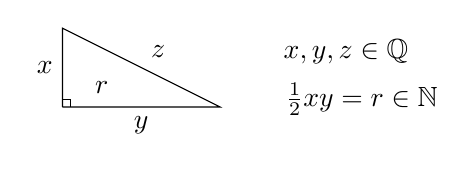
\begin{tikzpicture}[xscale=2, yscale=1]
		\coordinate (O) at (0,0);
		\coordinate (A) at (1,0);
		\coordinate (B) at (0,1);
		\coordinate (M) at (0.25, 0.25);
		\draw (O) -- node[auto,swap]{$y$} 
		(A) -- node[auto,swap]{$z$}
		(B) -- node[auto,swap]{$x$} (O);
		\draw (M) node[auto]{$r$};
		
		\coordinate (S) at (1.8, 0.7);
		\draw (S) node[auto]{$x,y,z\in\QQ$};
		\coordinate (N) at (1.9, 0.1);
		\draw (N) node[auto]{$\frac{1}{2}xy=r\in\NN$};
		\coordinate (X1) at (0,0.1);
		\coordinate (X2) at (0.05,0.1);
		\coordinate (X3) at (0.05,0);
		\draw (X1) -- (X2) -- (X3);
		\end{tikzpicture}
	\end{figure}\\
	Dit is een driehoek met zijn zijden in $\QQ$ en zijn oppervlakte in $\NN$. Dit betekent dus dat $r$ een congruent getal is.\\
	
	We bekijken nu dezelfde driehoek nadat we alle zijden vermigvuldigd hebben met een getal $s\in\NN$. Deze driehoek ziet er dan als volgt uit:
	\begin{figure}[h!]
		\centering
		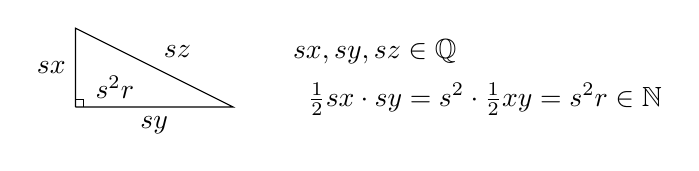
\begin{tikzpicture}[xscale=2, yscale=1]
		\coordinate (O) at (0,0);
		\coordinate (A) at (1,0);
		\coordinate (B) at (0,1);
		\coordinate (M) at (0.25, 0.25);
		\draw (O) -- node[auto,swap]{$sy$} 
		(A) -- node[auto,swap]{$sz$}
		(B) -- node[auto,swap]{$sx$} (O);
		\draw (M) node[auto]{$s^2r$};
		
		\coordinate (S) at (1.9, 0.7);
		\draw (S) node[auto]{$sx,sy,sz\in\QQ$};
		\coordinate (N) at (2.6, 0.1);
		\draw (N) node[auto]{$\frac{1}{2} sx \cdot sy = s^2 \cdot \frac{1}{2}xy = s^2r \in\NN$};
		\coordinate (X1) at (0,0.1);
		\coordinate (X2) at (0.05,0.1);
		\coordinate (X3) at (0.05,0);
		\draw (X1) -- (X2) -- (X3);
		\end{tikzpicture}
	\end{figure}\\
	We zien dat $s^2r\in\NN$ ook een congruent getal is, want de zijden van de driehoek bevinden zich in $\QQ$. Als we nu willen zoeken naar congruente getallen, kunnen we dus ook kijken naar alle kwadraatvrije\footnote{Een kwadraatvrij getal is een getal dat niet deelbaar is door een kwadraat groter dan $1$. Waarbij een kwadraat een getal $k\in\NN$ zodat $\sqrt{k}\in\NN$. \cite{Beukers}} getallen $m'\in\NN$. Namelijk: door het zojuist gegeven voorbeeld zien we dat we $r$ met een willekeurig kwadraat uit $\NN$ kunnen vermenigvuldigen zonder dat het zijn eigenschappen verliest, het is dan nog steeds een congruent getal.\\
	
	We kunnen dit proces ook omgekeerd uitvoeren. Stel we hebben een congruent getal $r$ dat niet kwadraatvrij is. Dit betekent dat er een kwadraat $s^2\in\NN$ bestaat waar we $r$ door kunnen delen. We kunnen de zijden van de driehoek delen door $s$. Nu hebben we een congruent getal $\frac{r}{s^2}$ met het bijbehorende Pythagore\"ische drietal $(\frac{x}{s}, \frac{y}{s}, \frac{z}{s})$. We kunnen dit proces net zolang herhalen totdat we een kwadraatvrij congruent getal hebben gevonden.\\

	We hebben nu dus gezien dat we alleen nog maar hoeven te kijken naar kwadraatvrije getallen. We nemen vanaf nu dus aan dat $n$ een kwadraatvrij congruent getal is. Dat betekent dat we al een stuk sneller door $\NN$ kunnen gaan om te kijken welke getallen congruent zijn. Sterker nog: er betstaat een algoritme dat voor elke $m'\in\NN$ checkt of er een Pythagore\"isch drietal bestaat zodat $m'$ de oppervlakte is van de driehoek die hoort bij dit Pythagore\"isch drietal. Als $m'$ congruent is, zet het algoritme $m'$ in een lijst. Helaas weten we niet of een getal dat niet in de lijst staat, ook daadwerkelijk geen congruent getal is. Het kan namelijk ook zo zijn dat het algoritme te lang moest zoeken naar een Pythagore\"isch drietal, waardoor het zoeken tijdig is afgebroken. Dit is dus nog steeds geen optimale manier om naar congruente getallen te zoeken. We zoeken dus eigenlijk nog steeds naar een formule die ons kan vertellen of een getal wel of niet congruent is. Daarvoor introduceren we eerst de stelling van Tunnell:
	\begin{theorem}\label{def:tunnell}
		\cite{Koblitz}[p.212, vertaald] (Tunnell, 1983) Als $n$ een kwadraatvrij en oneven (respectievelijk even) positief geheel getal is en $n$ is de oppervlakte van een rechthoekige driehoek met rationale zijden, dan
		\begin{align}
		\label{vgl:oneven} \#\{x,y,z\in\ZZ \mid n=2x^2+y^2+32z^2\} = \frac{1}{2} \#\{x,y,z\in\ZZ \mid n=2x^2+y^2+8z^2\}\\
		\notag \text{(respectievelijk} \\
		\label{vgl:even} \#\{x,y,z\in\ZZ \mid \frac{n}{2}=4x^2+y^2+32z^2\} = \frac{1}{2} \#\{x,y,z\in\ZZ \mid \frac{n}{2}=4x^2+y^2+8z^2\})
		\end{align}
		Omgekeerd, als het zwakke vermoeden van Birch en Swinnerton-Dyer waar is voor de elliptische krommen $E_n:y^2=x^3-n^2x$, dan, impliceren deze gelijkheden dat $n$ een congruent getal is.
	\end{theorem}
	\noindent Deze stelling zegt dat als $n$ een kwadraatvrij en congruent getal is, dan voldoet deze $n$ aan de vergelijkingen (\ref{vgl:oneven}) om (\ref{vgl:even}). Om te checken of een kwadraatvrij getal $m'\in\NN$ congruent is, willen we weten dat de stelling ook de andere kant op werkt. Dit kunnen we alleen aannemen als we het vermoeden van Birch en Swinnerton-Dyer aannemen, een vermoeden over elliptische krommen. Dit is voor nu te ingewikkeld, dus dit zullen we niet verder behandelen. Wat we nu in elk geval hebben is een formule om te bewijzen dat $m'$ niet congruent is en we kunnen zeer aannemelijk maken dat $n$ wel een congruent getal is.
	
	
	\section{Presentaties van congruente getallen}\label{sec:lotte}
	Zoals we in hoofdstuk \ref{sec:def} al gezien hebben, bestaan er verschillende definities voor een congruent getal. Wij gebruiken hier de meetkundige definitie, waarbij een congruent getal afhangt van een Pythagore\"isch drietal. We zullen hieronder eerst uitleggen wat een presentatie is, daarna zullen we een voorbeeld geven van een presentatie.
	
	\subsection{Wat is een presentatie?}\label{sec:presentaties}
	Het {\color{red}Het of Een?} Pythagore\"ische drietal dat bij een congruent getal hoort, heet de presentatie van het congruente getal. Zo is $(3,4,5)$ de presentatie van het congruente getal $6$. Oftewel,  de presentatie van een congruent getal $n$ is een drietal $(x,y,z)\in\QQ^3_{>0}$, zodat dit, met {\color{red}hier mist iets van een werkwoord zoals: het berkenen volgens} de meetkundige definitie, $n$ geeft.\\
	
	Het is belangrijk om hier op te merken dat een congruent getal meerdere presentaties heeft. Zo zijn $(21,20,29)$ en $(35,12,37)$ allebei presentaties van het congruente getal $210$ \cite{Oort}[p.9]. Sterker nog, ieder congruent getal heeft oneindig veel presentaties. We zullen dat {\color{red}dit} hieronder bewijzen.\\
	
	Om te beginnen, breiden we eerst de definitie van {\color{red}een / het begrip} presentatie uit. Het Pythagore\"ische drietal is \'e\'en versie van een presentatie. En hoewel deze heel praktisch is om congruente getallen te vinden, is deze niet handig voor ons bewijs. We gebruiken dus een andere {\color{red}moet hier niet ander staan?} soort presentatie, gebaseerd op de stelling van Euclides. Deze is van de vorm $((k,l),D,n)$; wat dit precies inhoudt, zal straks {\color{red}misschien straks vervangen door hieronder} duidelijk worden. Concreter gezegd: een presentatie is dat wat "bewijst" dat {\color{red}$n$?} een getal congruent is.\\
	
	Om deze nieuwe presentatie te begrijpen, hebben we de volgende stelling nodig:
	\begin{theorem}\label{def:euclides}
		\cite{Oort}[p.8] (Euclides) Als $(x,y,z)$ een primitief Pythagore\"isch drietal is met $x$ oneven, dan zijn er getallen $k,l\in\ZZ_{>0}$ met $k>l$, $\ggd(k,l)=1$ en $k+l$ oneven zodat
		\begin{equation*}
			x=k^2-l^2,\qquad y=2kl,\qquad z=k^2+l^2.
		\end{equation*}
	\end{theorem}
	\noindent Deze stelling verklaart alvast {\color{red}Ik zou dit anders verwoorden. Zoiets als: We weten nu dus wat de $k$ en $l$ betekenen} de $k$ en $l$ in onze nieuwe presentatie $((k,l),D,n)$.\\
	
	De {\color{red}variabelen} $D$ en $n$ zijn allebei positieve gehele getallen, afhankelijk van $k$ en $l$. Dat zit zo {\color{red}Volgens de volgende relatie (ofzoiets)}: $n=\frac{kl(k^2-l^2)}{D^2}$, waarbij $n$ een kwadraatvrij congruent getal is en $D$ is het grootste positieve gehele getal waarvan het kwadraat een deler is van $kl(k^2-l^2)$. Dus $((k,l),D,n)$ is een presentatie van $n$.\\
	
	Nu we weten wat de presentatie $((k,l),D,n)$ inhoudt, kunnen we beginnen met het bewijzen van de volgende stelling.	
	\begin{theorem}
		Elk congruent getal heeft oneindig veel presentaties.
	\end{theorem}
	
	\begin{proof}
		We defini\"eren eerst:
		\begin{equation*}
			U:=z^2=(k^2+l^2)^2, \qquad V:=2xy=2\cdot(k^2-l^2)\cdot 2kl
		\end{equation*}
		Met $U$ en $V$ kunnen we een andere presentatie vinden voor ons congruente getal. Dat doen we als volgt:
		\begin{align*}
			UV (U - V) (U + V) &= z^2 \cdot 2xy (z^2 - 2xy) (z^2 + 2xy)\\
			&= z^2 \cdot 2xy (x^2 + y^2 - 2xy) (x^2 + y^2 + 2xy)\\
			&= 2xy \cdot z^2 (x - y)^2 (x + y)^2\\
			&= 2 (k^2-l^2) \cdot 2kl (k^2+l^2)^2 (x - y)^2 (x + y)^2\\
			&= (2 (k^2+l^2) (x-y) (x+y))^2 \cdot kl (k^2-l^2)\\
			&= (2 z (x - y) (x + y))^2 \cdot D^2n\\
			&= (2 z D (x - y) (x + y))^2 \cdot n
		\end{align*}
		
		We hebben zo dus een nieuwe presentatie gevonden voor $n$, die we $((p,q),E,n)$ noemen, met het bijbehorend Pythagor\"isch drietal $(a,b,c)$.\footnote{Hierbij hebben $p$ en $q$ dezelfde rol als $k$ en $l$, en $E$ vervangt $D$. Het congruente getal verandert niet, en is dus nog steeds $n$. $(a,b,c)$ {\color{red}Begin een zin nooit met een variable.} is het bijbehorende Pythagore\"isch drietal, waarbij geldt dat $a=p^2-q^2$, $b=2pq$ en $c=p^2+q^2$.} {\color{red}Ik zou deze footnote weglaten en het lekker in de tekst zetten, want het is belangrijk voor het stuk.} Zowel $p$ en $q$ als $(a,b,c)$ voldoen uiteraard aan de eisen die gesteld zijn in de stelling van Euclides.\\
		
		Dat de gevonden presentatie niet gelijk is aan de originele, is te zien aan de constante $E$. Er geldt namelijk:
		\begin{align*}
			E &= | 2 z D (x-y) (x+y) | \\
			&= 2 D \cdot | z (x-y) (x+y) | \\
			&\geq 2 D \\
			&> D.
		\end{align*}
		Dus $E > D$.\\
		
		We kunnen nu vervangers defini\"eren voor $U$ en $V$, behorende bij de nieuwe presentatie. We noemen deze $U'$ en $V'$. Ze zijn op dezelfde manier gedefini\"eerd, namelijk $U':=c^2=(p^2+q^2)^2$ en $V':=2ab=2\cdot(p^2-q^2)\cdot2pq$.\\
		
		We kunnen dezelfde berekeningen doen met $U'$ en $V'$. We krijgen dan weer een andere presentatie. Belangrijker nog, we krijgen de nieuwe constante $F$ {\color{red}cool, wat doet die constante dan? (mention even dat deze E vervangt oid)} waarvoor geldt: $F=|2 c E (a-b) (a+b)|.$ Uiteraard geldt dan dat $F > E$ {\color{red}Ik zou die align hierboven veranderen in een equation zonder sterretje. Je kan binnen de equation een split gebruiken om het nog wel op verschillende regels te zetten. Dan kan je die een label geven en hier referen dat op dezelfde manier als in (.) geldt dat F>E}.\\
		
		We kunnen de procedure dus {\color{red}Ik zou deze dus weghalen en zoiets zeggen als: We kunnen deze procedure oneindig vaak herhalen, wat ons dan oneindig veel presentatie opleverd (ofzoiets)} oneindig vaak herhalen, steeds met een andere presentatie als uitkomst. Dat betekent dus dat voor ons congruente getal $n$ (en dus ieder congruent getal $n$) oneindig veel presentaties bestaan.
	\end{proof}
	
	\subsection{Een voorbeeld van een presentatie}
	We hebben in hoofdstuk \ref{sec:presentaties} {\color{red}Ik zou denk ik zeggen ``in de paragraaf hiervoor".} een bewijs geleverd dat er oneindig veel presentaties bestaan, maar we hebben nog niet gezien hoe deze methode in de praktijk werkt. Dat gaan we hier doen{\color{red}zullen we nu laten zien}, voor het congruente getal 210.\\
	
	Als eerste willen we uiteraard {\color{red}ik zou de uiteraard weglaten} controleren of 210 inderdaad een congruent en kwadraatvrij getal {\color{red}kwadraatvrij congruent getal} is. Dat het congruent is, weten we al {\color{red}door de eerder gegeven presentaties (rest weglaten)}. Immers, eerder zijn al twee presentaties gegeven, namelijk $(21,20,29)$ en $(35,12,37)$. Dat 210 ook kwadraatvrij is, is {\color{red}kunnen we nagaan door (is mooier dan twee keer is achter elkaar) }na te gaan door het getal op te splitsen in priemfactoren. Voor 210 geldt: {\color{red}je kan dit weglaten en de punt vervangen door een ; } $210 = 2 \cdot 3 \cdot 5 \cdot 7$. Geen enkel getal komt dubbel voor, dus is 210 ook {\color{red}ook weglaten} kwadraatvrij.\\
	
	We kennen al twee presentaties voor 210. We kiezen ervoor om $(21,20,29)$ te gebruiken.\\
	
	Allereerst willen we een presentatie van de vorm $((k,l),D,n)$ vinden. De constante $n=210$ weten we al, dus resteren $k$, $l$ en $D$. We kunnen $k$ en $l$ berekenen door de formules $x = k^2 - l^2$, $y = 2kl$ en $z = k^2 + l^2$. {\color{red}De zin die hierop volgt zou ik weglaten en tussen de vergelijkingen stoppen, op de plek waar je zegt Nu resteert alleen D nog, Deze kunnen we bereken met ....} De laatste constante, $D$, berekenen we met de formule $n = kl \cdot \frac{k^2-l^2}{D^2}$.\\
	
	\noindent We rekenen eerst $k$ uit:
	\begin{equation*}
		k^2 = \frac{1}{2}((k^2-l^2)+(k^2+l^2)) = \frac{1}{2} (x+z) = \frac{1}{2} (21+29) = 25.
	\end{equation*}
	Dus $k = \sqrt{25} = 5$. Vervolgens kunnen we ook $l$ uitrekenen:
	\begin{equation*}
		l = \frac{y}{2k} = \frac{20}{2 \cdot 5} = 2.
	\end{equation*}
	Nu resteert alleen $D$ nog:
	\begin{align*}
		n &= kl \cdot \frac{k^2-l^2}{D^2}.
		\intertext{Als we dit invullen, krijgen we:}
		210 &= 5 \cdot 2 \cdot \frac{5^2-2^2}{D^2} = \frac{210}{D^2}.
	\end{align*}
	Dus $D = \sqrt{1} = 1$. De gezochte presentatie is dus $((5,2),1,210)$. Hiermee kunnen we weer een nieuwe variabele $E$ vinden, die de sleutel vormt voor een nieuwe presentatie. Hiervoor gebruiken we een formule uit het bewijs: $E = |2 z D  (x - y) (x+y)|$. Zo blijkt dan dat $E = |2 \cdot 29 \cdot 1 \cdot (21-20) (21+20)| = 2378$. De rest van de presentatie zal ook vele malen groter zijn dan het origineel, doordat {\color{red}omdat} $E$ zo groot is.\\
	
	Dezelfde stappen kunnen we uitvoeren voor andere kwadraatvrije congruente getallen. De andere presentatie van {\color{red}$n=$ of het congruente getal} 210, {\color{red}namelijk:} $(35,12,37)$, blijkt dan {\color{red}dan weglaten} $((6,1),1,210)$ te zijn en geeft $E = 79994$. De eerdergegeven {\color{red}zijn dit niet twee woorden?} presentatie van {\color{red}$n=$ of het congruente getal} 6, {\color{red}zelfde verhaal} $(3,4,5)$, levert dan {\color{red}de presentatie} $((2,1),1,6)$ en $E = 70$ op.
	
	
	\section{Samenvatting}
	
	
	\bibliographystyle{plain}
	\bibliography{bib}
\end{document}
